\chapter{Introduzione}



La generazione di immagini da prompt testuali è atta alla creazione di rappresentazioni visive realistiche e coerenti a partire da descrizioni linguistiche, 
avvalendosi di modelli generativi.

Stante la complessità che la generazione di immagini e la comprensione del testo \emph{eo ipso} rappresentano, 
la generazione di immagini da prompt testuali, essendo il combinato disposto delle due, presenta un'ulteriore difficoltà: 
il passaggio da un dominio di rappresentazione all'altro per convertire esplicite relazioni testuali tra entità, in immagini consistenti con il significato del testo. 

Inoltre, un buon modello deve poter mescolare concetti e stili che non ha mai visto prima per generare immagini inedite.
Ad esempio, non esistono ritratti di Kim Jong-Un in camera da letto che stringe degli orsacchiotti, 
ma, ricorrendo a tecnologie che sottendono l'addestramento di reti neurali, è possibile creare una siffatta immagine (Figura~\ref{fig:midjourney_figures}).
Inoltre, sarebbe auspicabile che il modello desumesse accuratamente il modo in cui gli oggetti nell'immagine generata si relazionano tra loro, 
in base alla semantica del messaggio testuale e \emph{come} viene conferito significato alle parole attraverso il contesto~\cite{fosterGenerativeDeepLearning2023}.
Ad esempio, l'immagine di “una persona con un salvagente che galleggia in mare” dovrebbe apparire molto dissimile da quella di 
“una persona con un salvagente in un mare di gente”. 

\smallskip
\noindent In questa trattazione si approfondirà la sola parte relativa alla generazione di immagini, piuttosto che il meccanismo 
con cui si estrapola la semantica da un blocco testuale e la conseguente creazione di un'immagine che ne rifletta il contenuto.

\noindent In particolare, il lavoro è così ripartito:
\begin{itemize}
\item nel \hyperref[chap:generative_modeling]{Capitolo 2} si chiarisce cosa si intenda per modellazione generativa e la si confronta con la modellazione discriminativa. Inoltre, si riporta una tassonomia di modelli generativi.
\item nel \hyperref[chap:diff_models]{Capitolo 3} si illustra dettagliatamente una particolare tipologia di modelli di diffusione, che ha rappresentato un contributo pionieristico nell'ambito della modellazione generativa:
i modelli probabilistici di diffusione del rumore (\emph{Denoising Diffusion Probabilistic Models}) (DDPM). Tali modelli rimuovono gradualmente il rumore 
da una versione corrotta di una data immagine, pervenendo, con l'ausilio di una rete neurale, ad una stima della distribuzione dell'immagine originale.
In appendice~\ref{appendix:probability_statistics} si riportano alcune nozioni di base di probabilità e statistisca a supporto della discussione dei suddetti modelli, 
mentre nelle appendici~\ref{appendix:details_loss} e~\ref{appendix:unet} se ne forniscono, rispettivamente, i dettagli matematici e architetturali.
\end{itemize}
 


\begin{figure}
    \centering
    \subfloat[][Prompt:\emph{“Pope Francis playing dj console, wearing dj headphones”}]
    {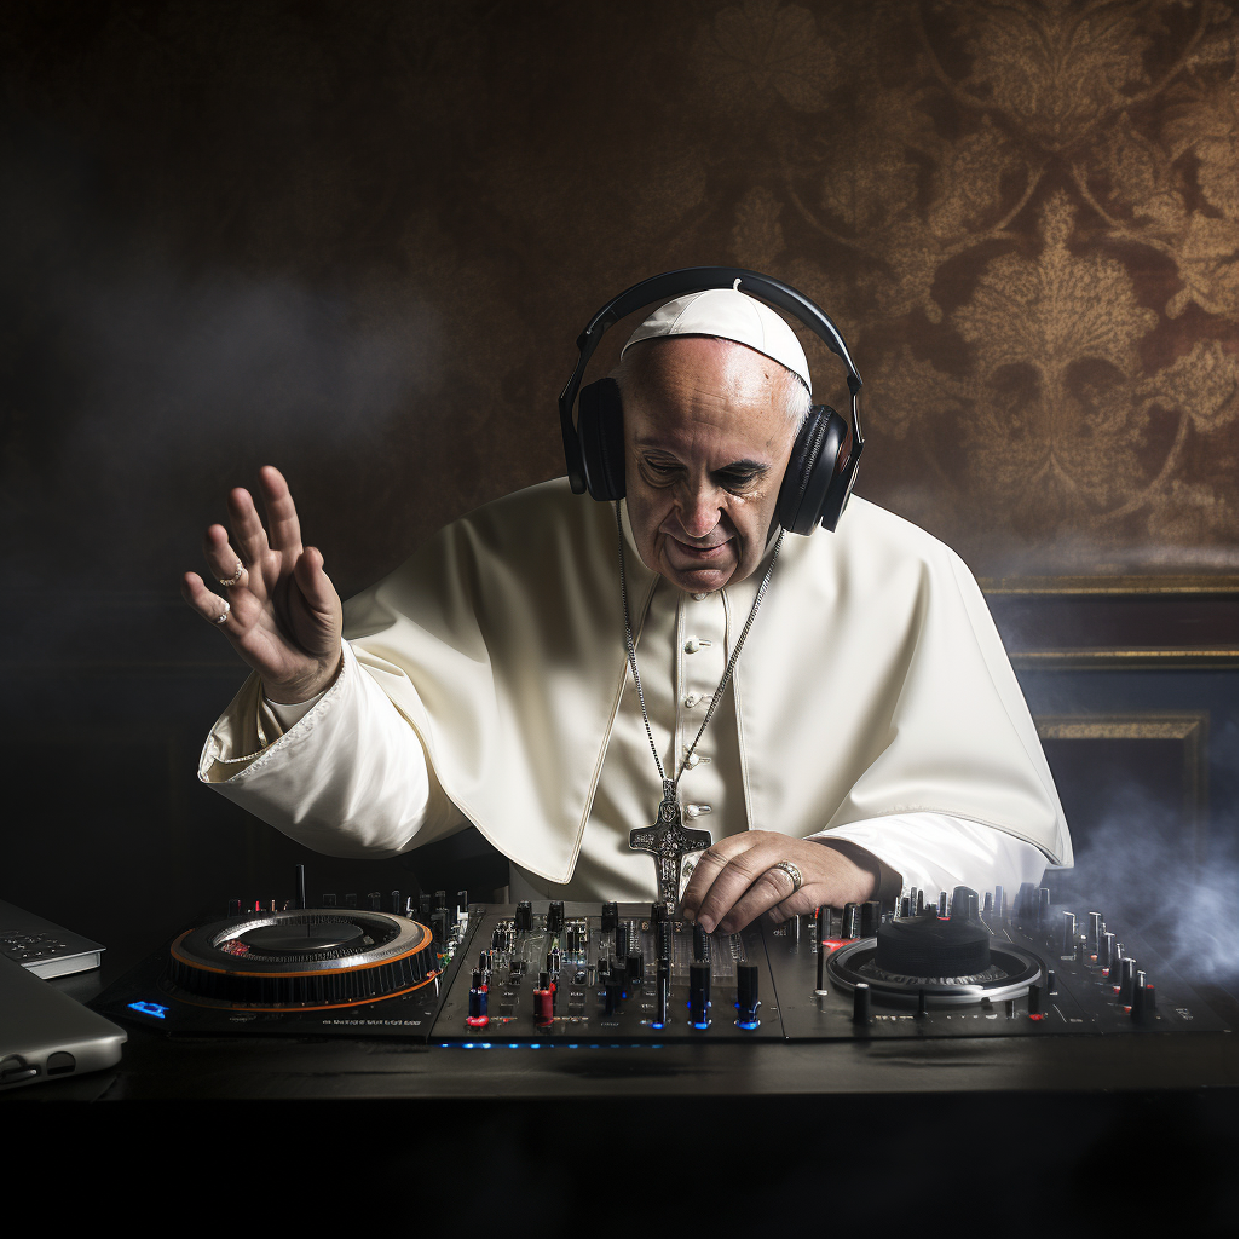
\includegraphics[width=.33\textwidth]{Pope_Francis}} \quad
    \subfloat[][Prompt:\emph{“Kim Jong-Un wearing hello kitty pattern pajama in bedroom holding a big hello kitty peluche”}]
    {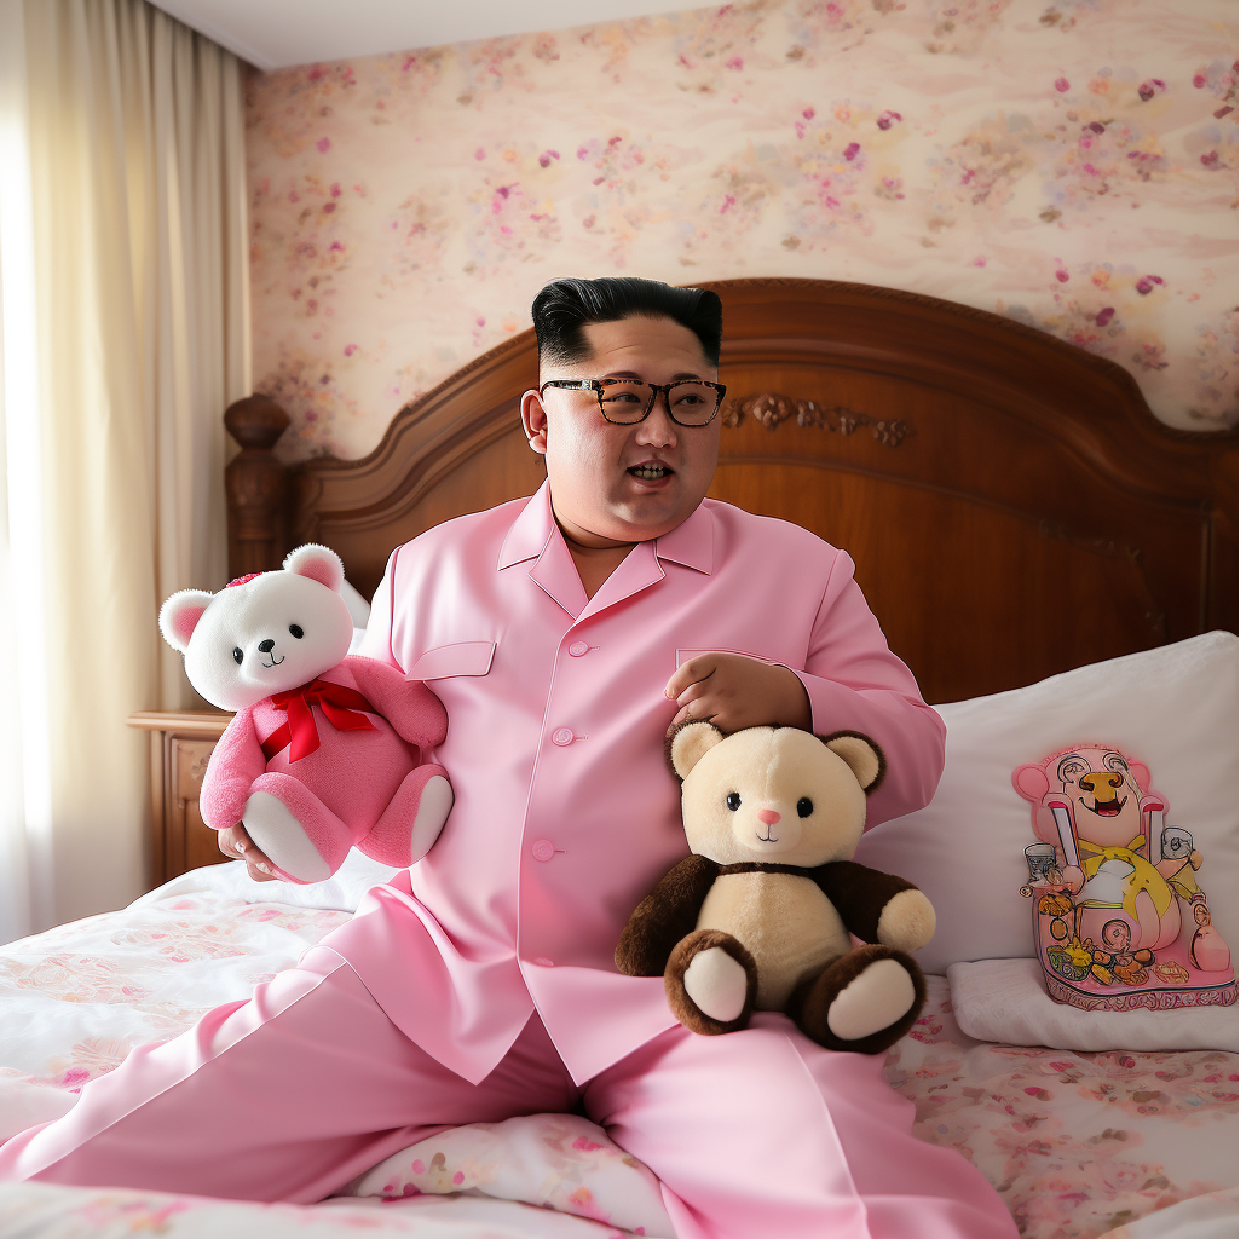
\includegraphics[width=.33\textwidth]{Kim_Jong_Un}} \\
    \subfloat[][Prompt:\emph{“Trump escorted by police officers”}]
    {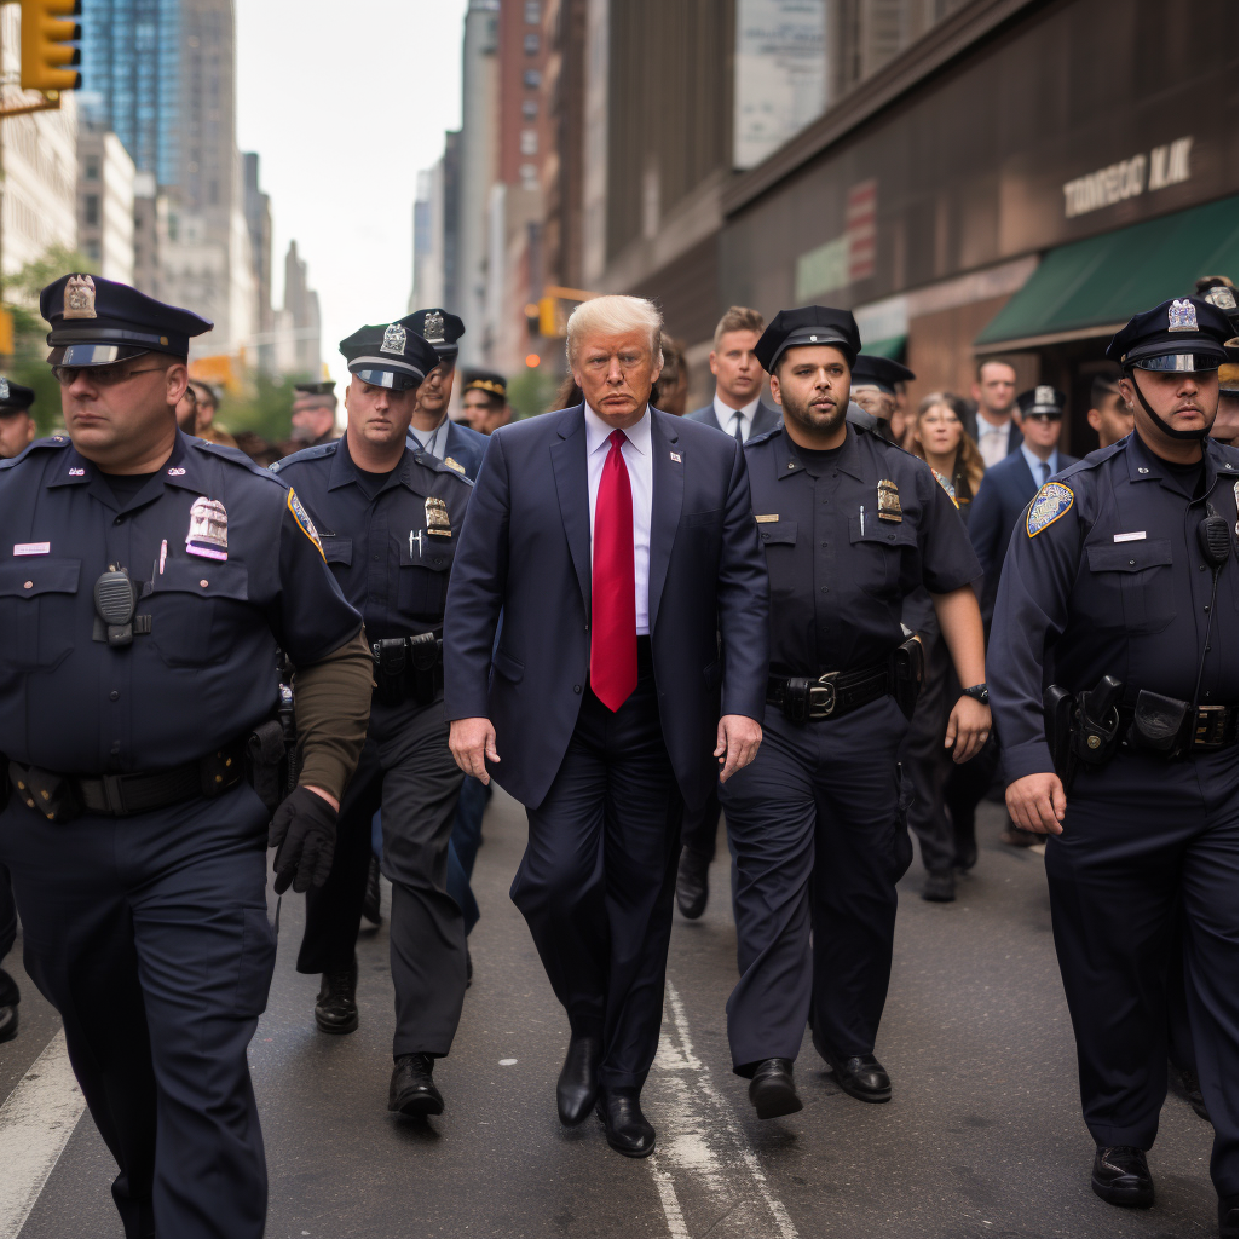
\includegraphics[width=.33\textwidth]{Trump}} \quad
    \subfloat[][Prompt:\emph{“Trump in prison doing bodybuilding”}]
    {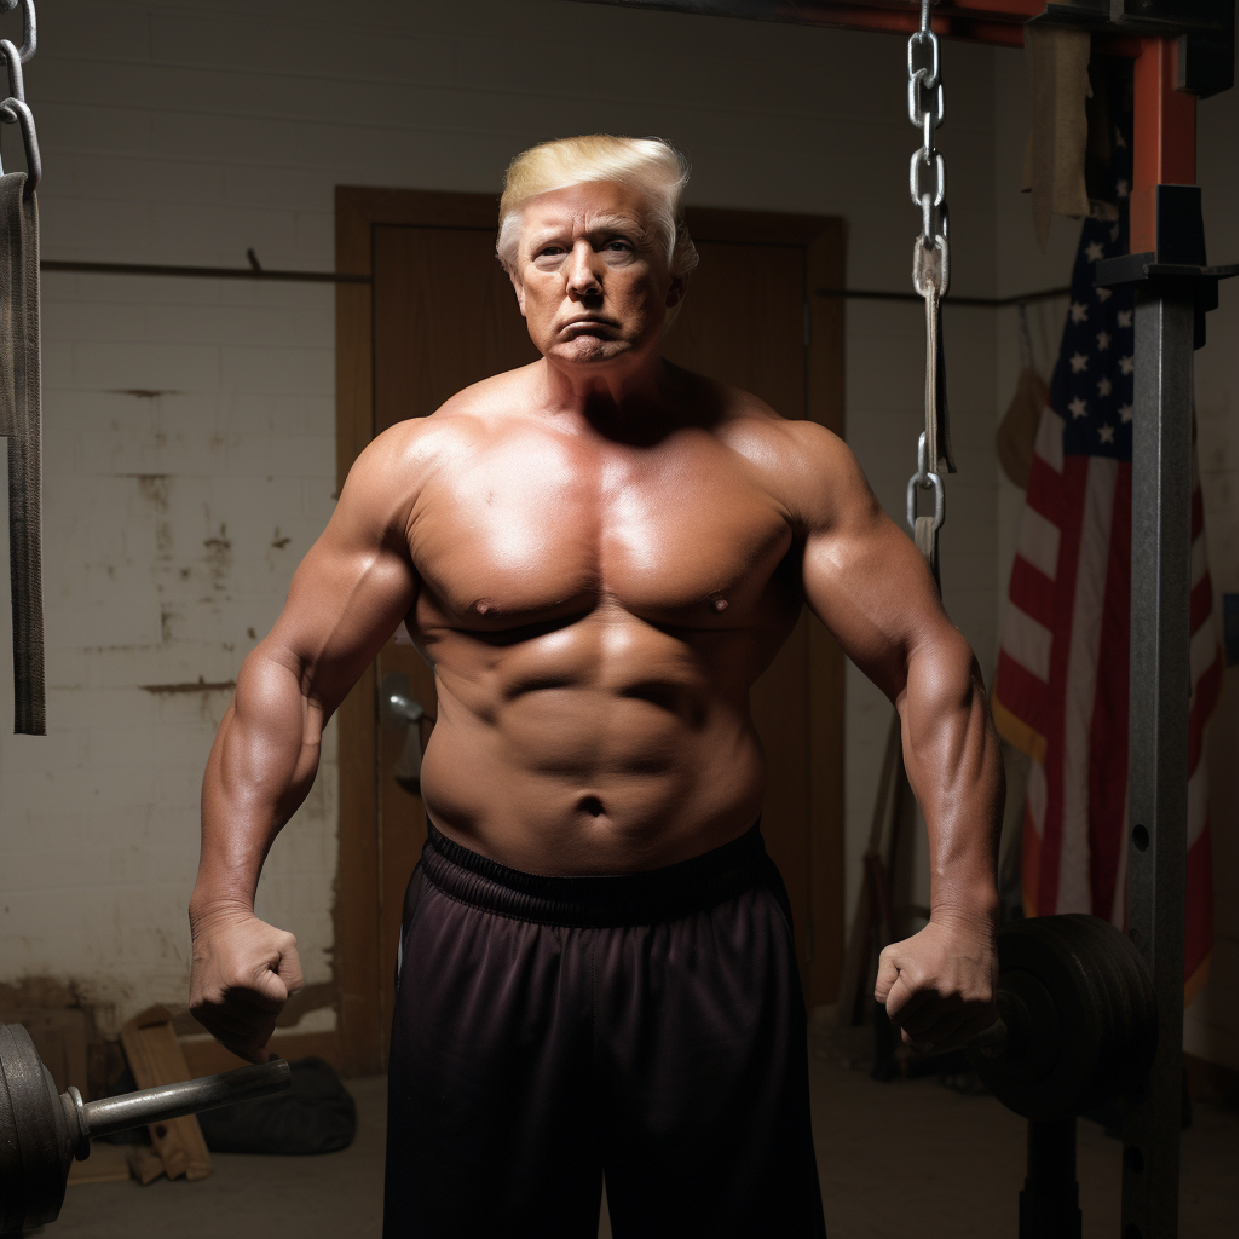
\includegraphics[width=.33\textwidth]{Trump_in_prison_doing_bodybuilding}}
    \caption{Immagini da me create con \emph{Midjourney}~\cite{Midjourney}, corredate dai prompt testuali originali in lingua inglese.}
    \label{fig:midjourney_figures}
\end{figure}
